\thispagestyle{fancy}
\vspace*{40 pt}
\subsection{Tela ajustes impressoras}\label{telaAjustesImpressoras}
Esta tela é acessada pelo botão "IMP" ou "IMP X" sendo X o número da impressora atualmente selecionada de qualquer uma das telas de ajustes.
\vspace*{\fill}
\begin{figure}[h]
  \centering
  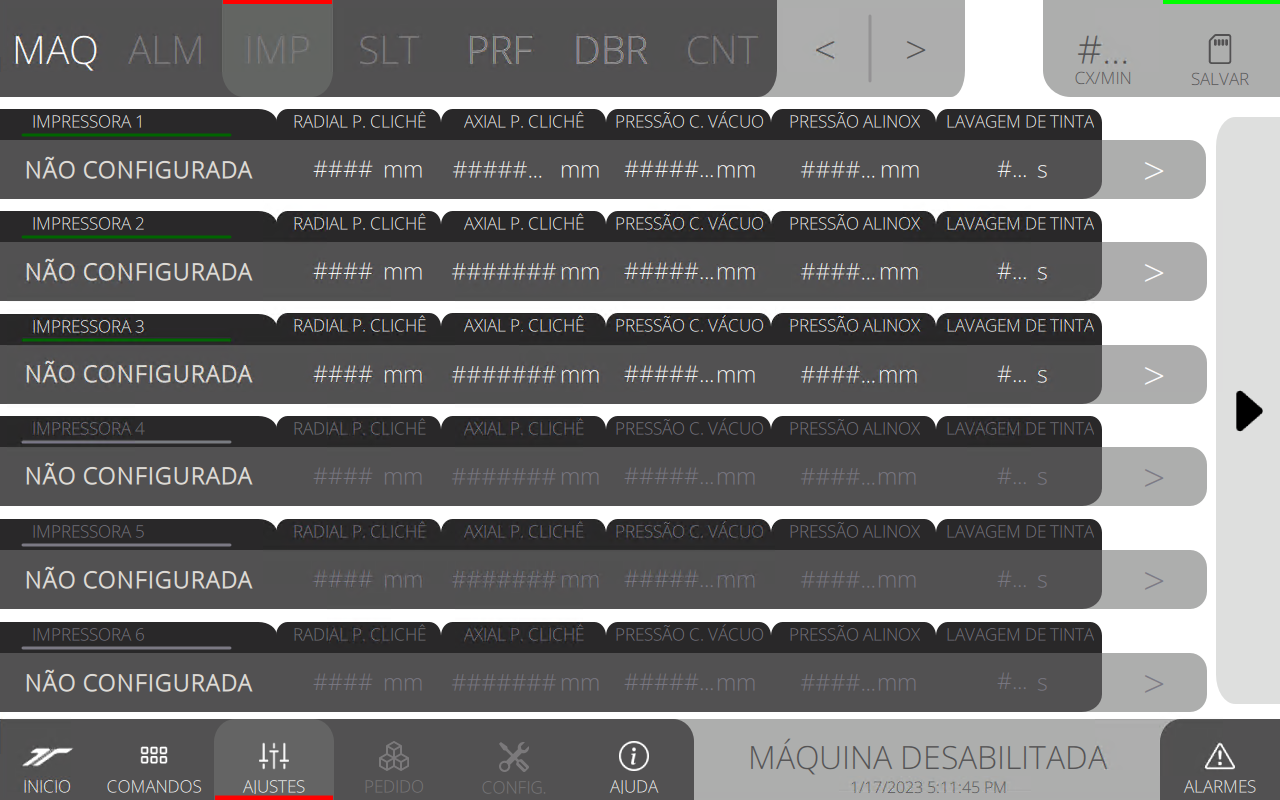
\includegraphics[width=576px,height=360px]{src/imagesFlexo/04-printter/01-printters/settings/e-Tela-Principal.png}
\end{figure}
\vspace*{\fill}

\newpage
\thispagestyle{fancy}
\vspace*{40 pt}
\subsubsection{\small{Visualização cor impressora}}\label{telaAjustesImpressorasVisualizacaoCorImpressora}
\vspace*{\fill}
\begin{figure}[h]
  \centering
  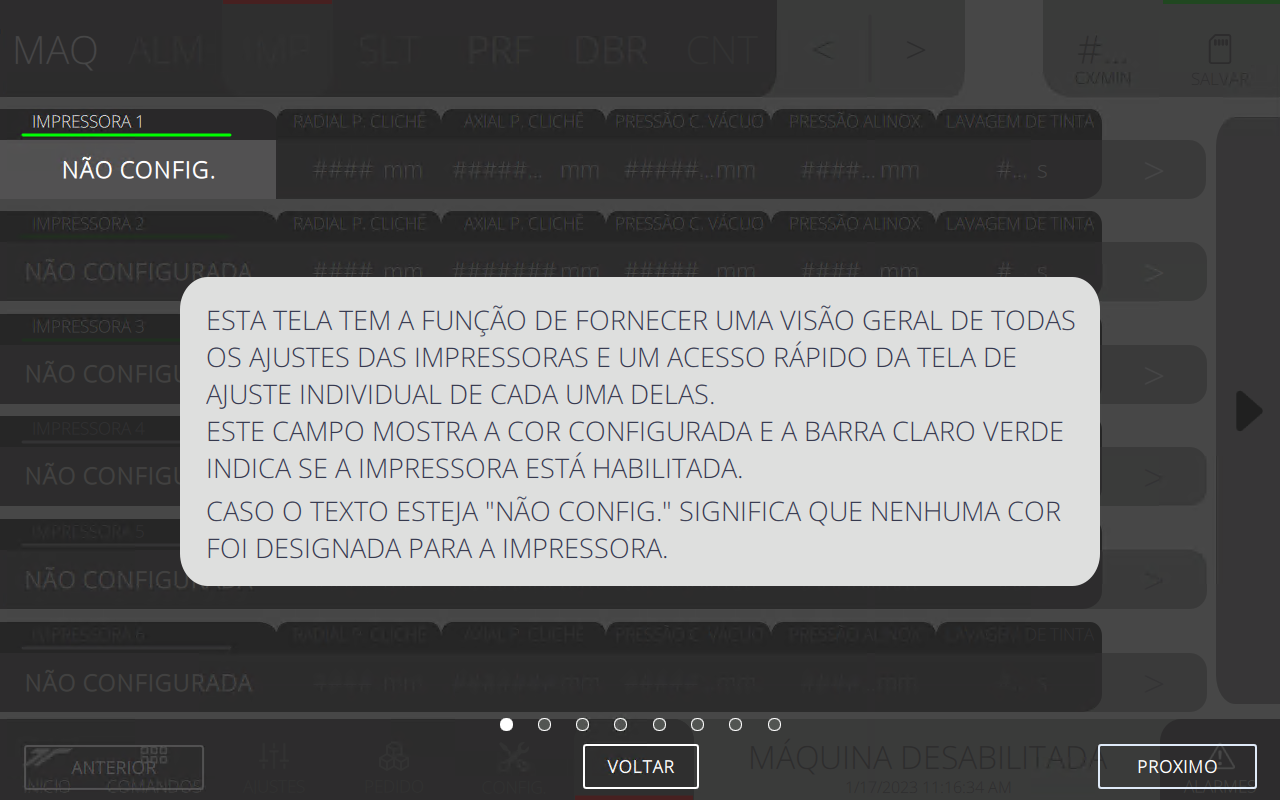
\includegraphics[width=576px,height=360px]{src/imagesFlexo/04-printter/01-printters/settings/e-1.png}
\end{figure}
\vspace*{\fill}

\newpage
\thispagestyle{fancy}
\vspace*{40 pt}
\subsubsection{\small{Visualização se a aproximação do anilox está bloqueada}}\label{telaAjustesImpressorasVisualizacaoSeAproximacaoDoAniloxEstaBloqueada}
\vspace*{\fill}
\begin{figure}[h]
  \centering
  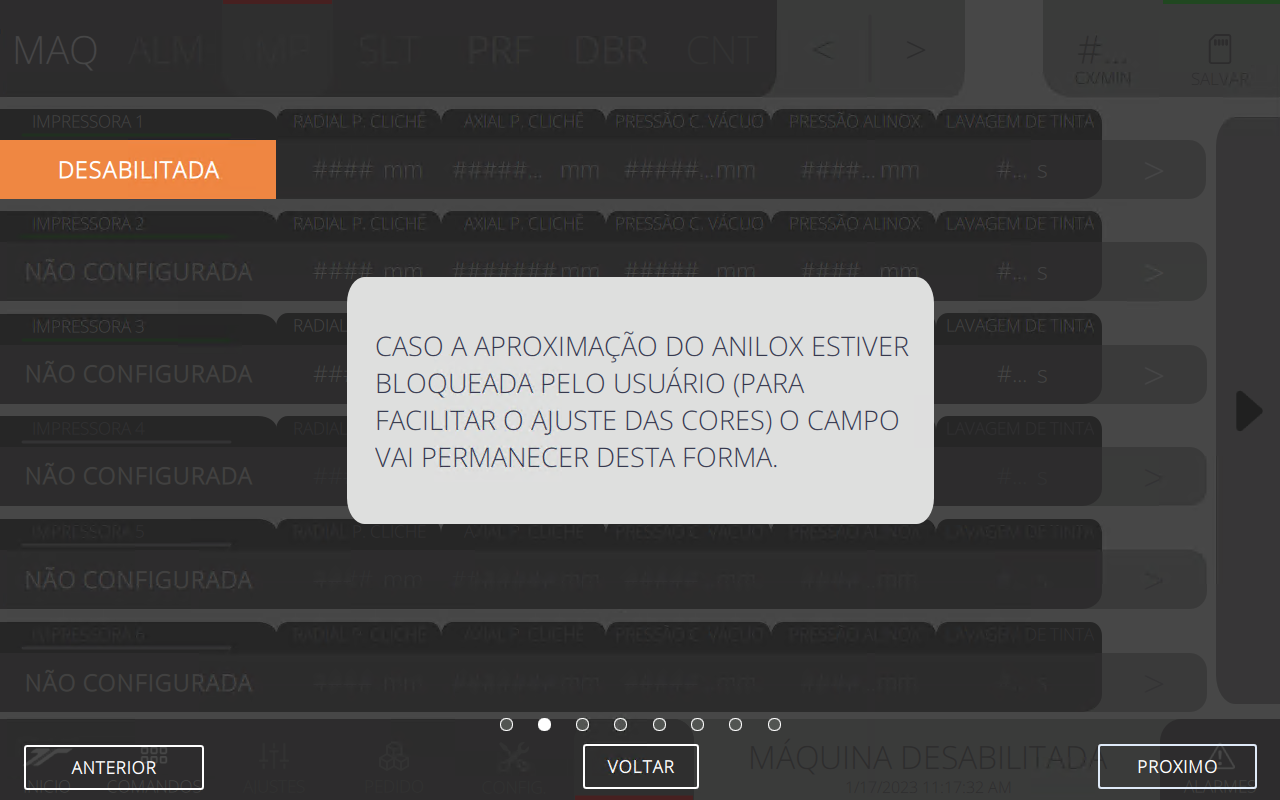
\includegraphics[width=576px,height=360px]{src/imagesFlexo/04-printter/01-printters/settings/e-2.png}
\end{figure}
\vspace*{\fill}

\newpage
\thispagestyle{fancy}
\vspace*{40 pt}
\subsubsection{\small{Visualização registro atual do clichê}}\label{telaAjustesImpressorasVisualizacaoRegistroAtualDoCliche}
\vspace*{\fill}
\begin{figure}[h]
  \centering
  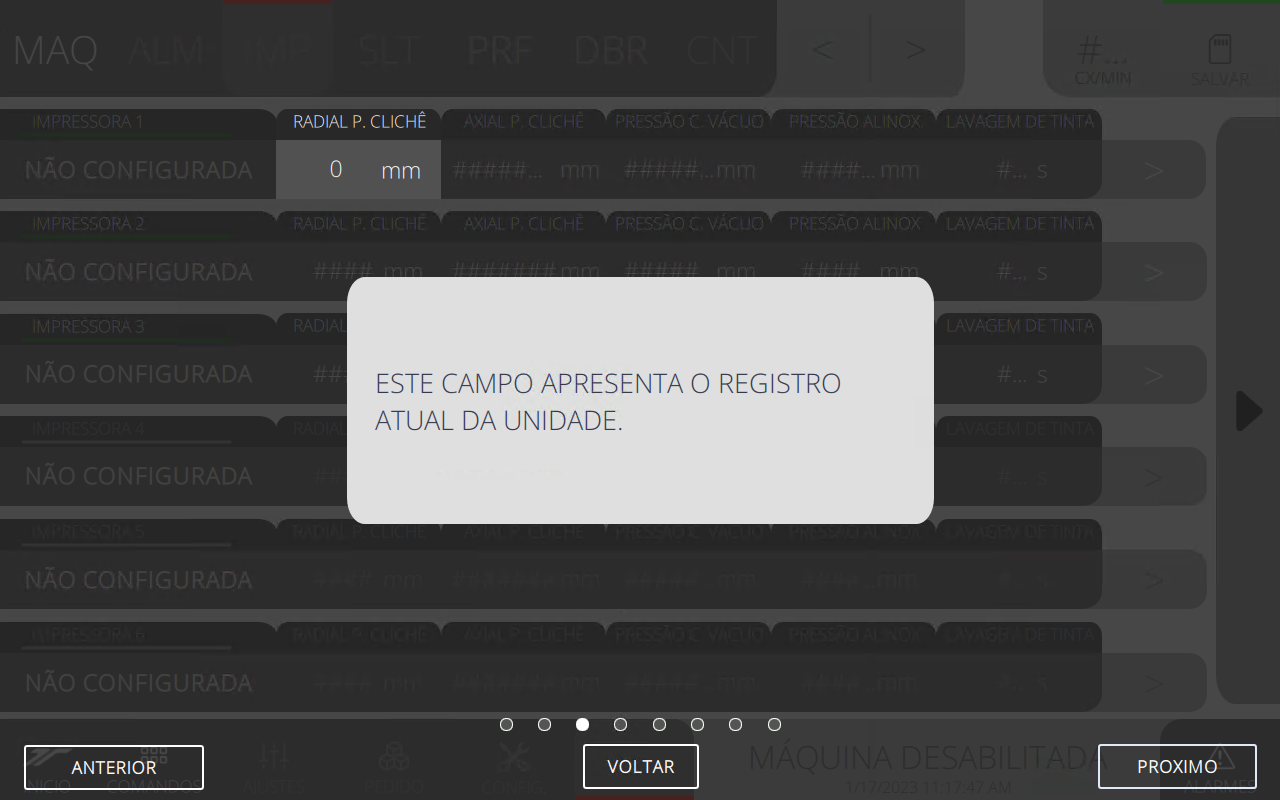
\includegraphics[width=576px,height=360px]{src/imagesFlexo/04-printter/01-printters/settings/e-3.png}
\end{figure}
\vspace*{\fill}

\newpage
\thispagestyle{fancy}
\vspace*{40 pt}
\subsubsection{\small{Visualização posição axial do porta clichê}}\label{telaAjustesImpressorasVisualizacaoPosicaoAxialDoPortaCliche}
\vspace*{\fill}
\begin{figure}[h]
  \centering
  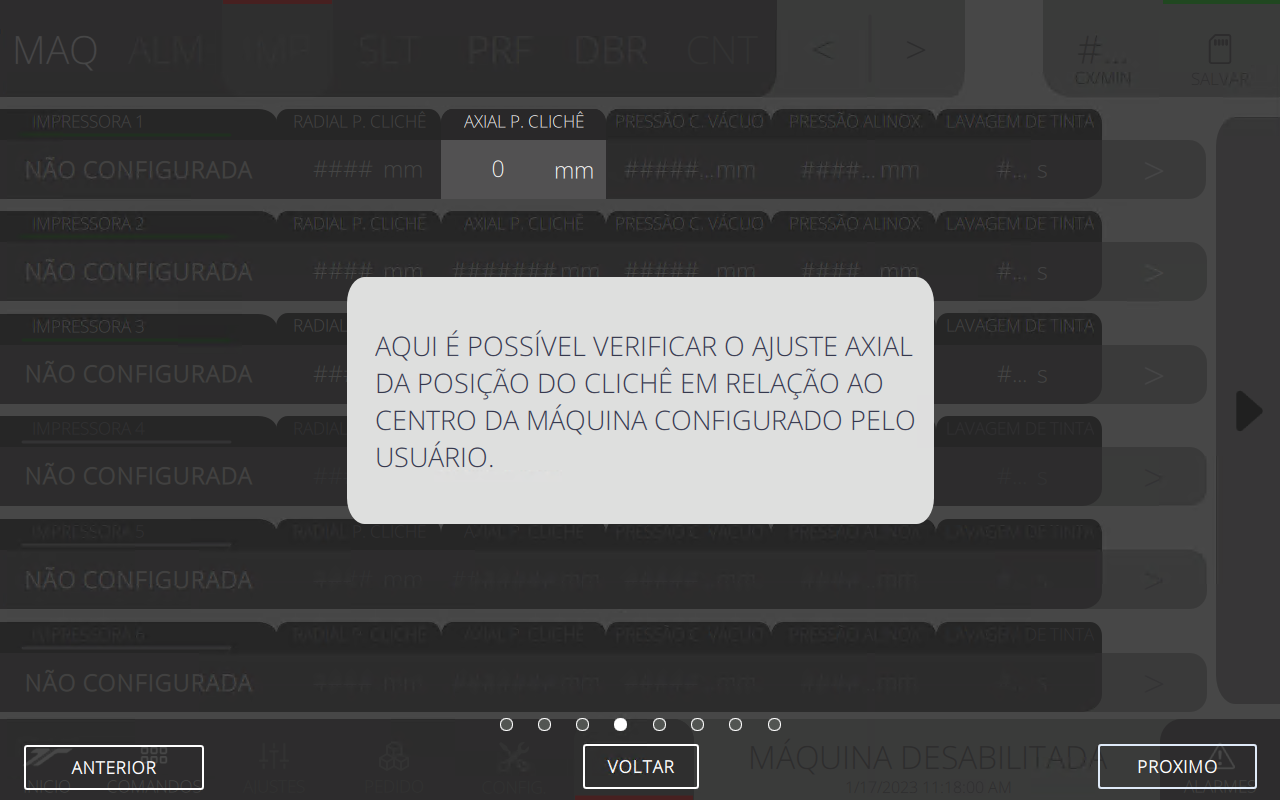
\includegraphics[width=576px,height=360px]{src/imagesFlexo/04-printter/01-printters/settings/e-4.png}
\end{figure}
\vspace*{\fill}

\newpage
\thispagestyle{fancy}
\vspace*{40 pt}
\subsubsection{\small{Visualização pressão da caixa de vácuo}}\label{telaAjustesImpressorasVisualizacaoPressaoDaCaixaDeVacio}
\vspace*{\fill}
\begin{figure}[h]
  \centering
  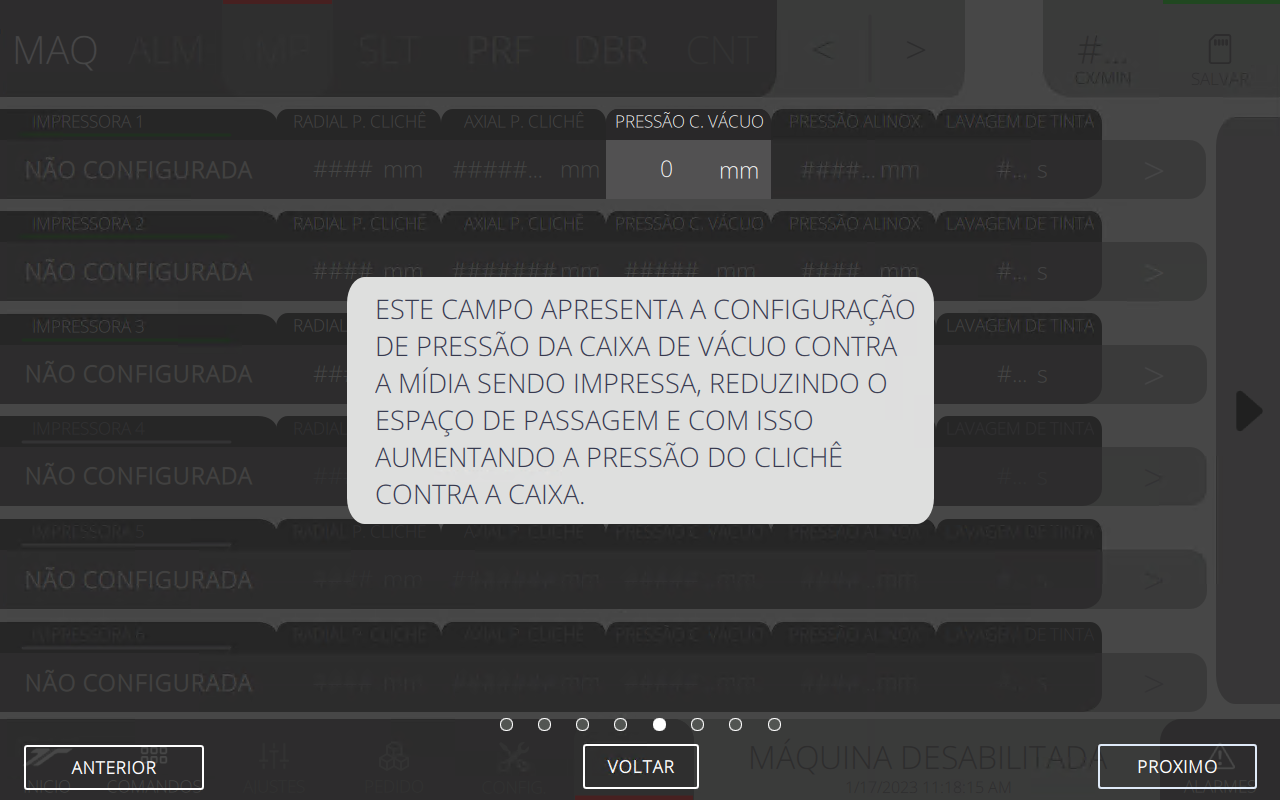
\includegraphics[width=576px,height=360px]{src/imagesFlexo/04-printter/01-printters/settings/e-5.png}
\end{figure}
\vspace*{\fill}

\newpage
\thispagestyle{fancy}
\vspace*{40 pt}
\subsubsection{\small{Visualização pressão do rolo anilox}}\label{telaAjustesImpressorasVisualizacaoPressaoDoRoloAnilox}
\vspace*{\fill}
\begin{figure}[h]
  \centering
  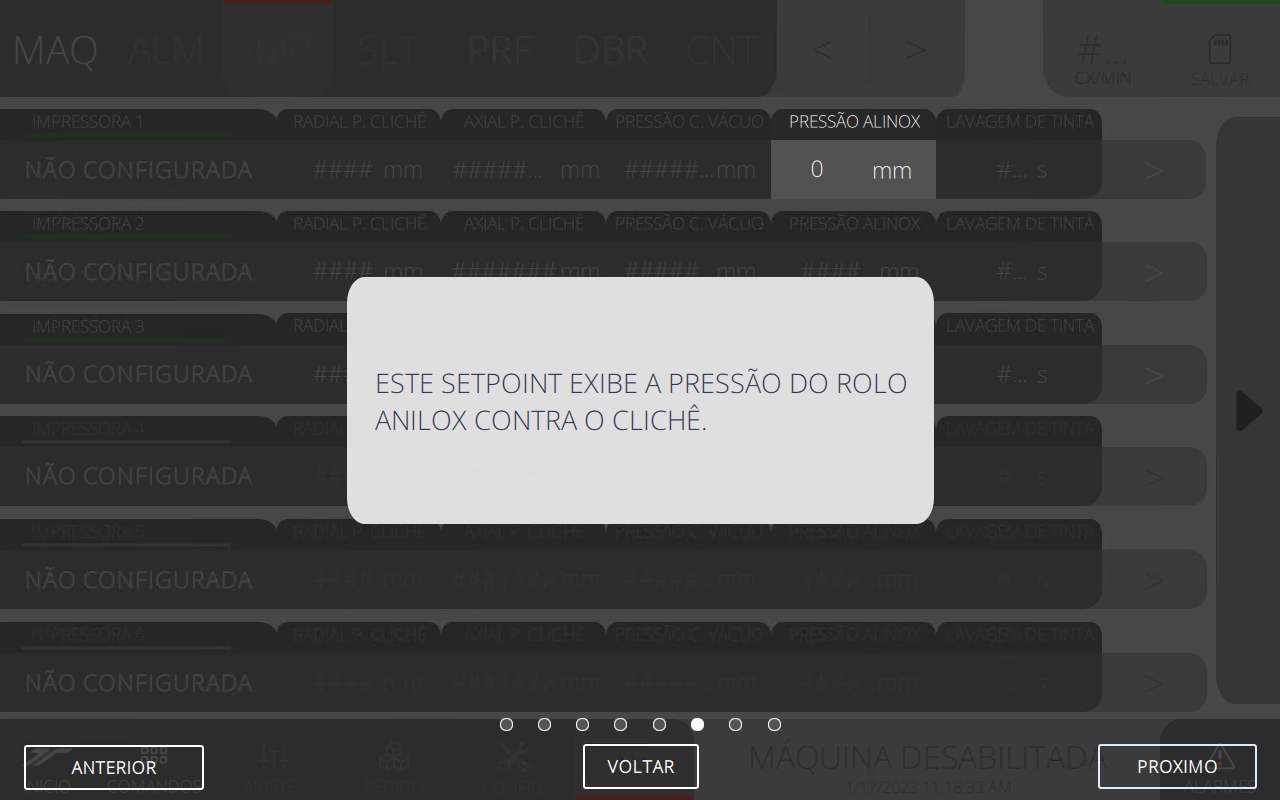
\includegraphics[width=576px,height=360px]{src/imagesFlexo/04-printter/01-printters/settings/e-6.png}
\end{figure}
\vspace*{\fill}

\newpage
\thispagestyle{fancy}
\vspace*{40 pt}
\subsubsection{\small{Tempo de lavagem de tinta}}\label{telaAjustesImpressorasTempoDeLavagemDeTinta}
\vspace*{\fill}
\begin{figure}[h]
  \centering
  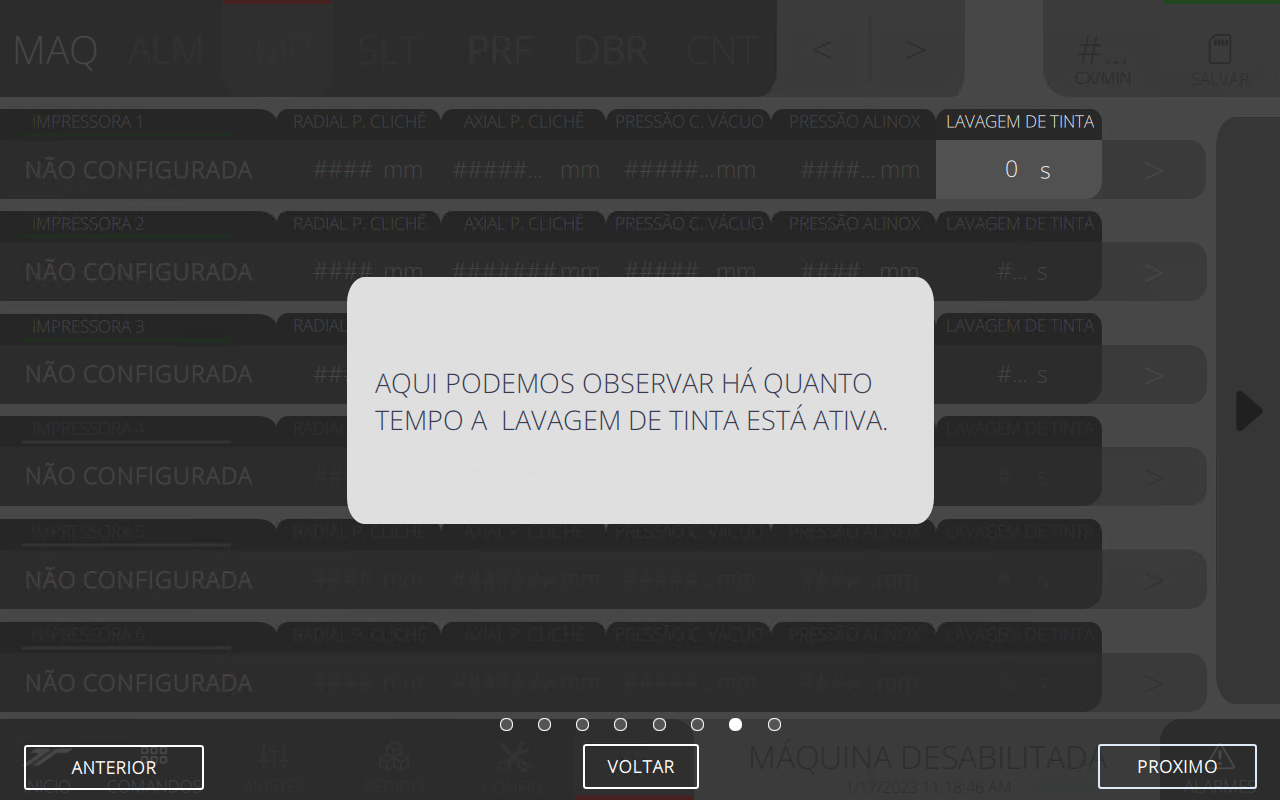
\includegraphics[width=576px,height=360px]{src/imagesFlexo/04-printter/01-printters/settings/e-7.png}
\end{figure}
\vspace*{\fill}

\newpage
\thispagestyle{fancy}
\vspace*{40 pt}
\subsubsection{\small{Botão de atalho para tela de ajustes da impressora}}\label{telaAjustesImpressorasBotaoDeAtalhoParaTelaDeAjustesDaImpressora}
\vspace*{\fill}
\begin{figure}[h]
  \centering
  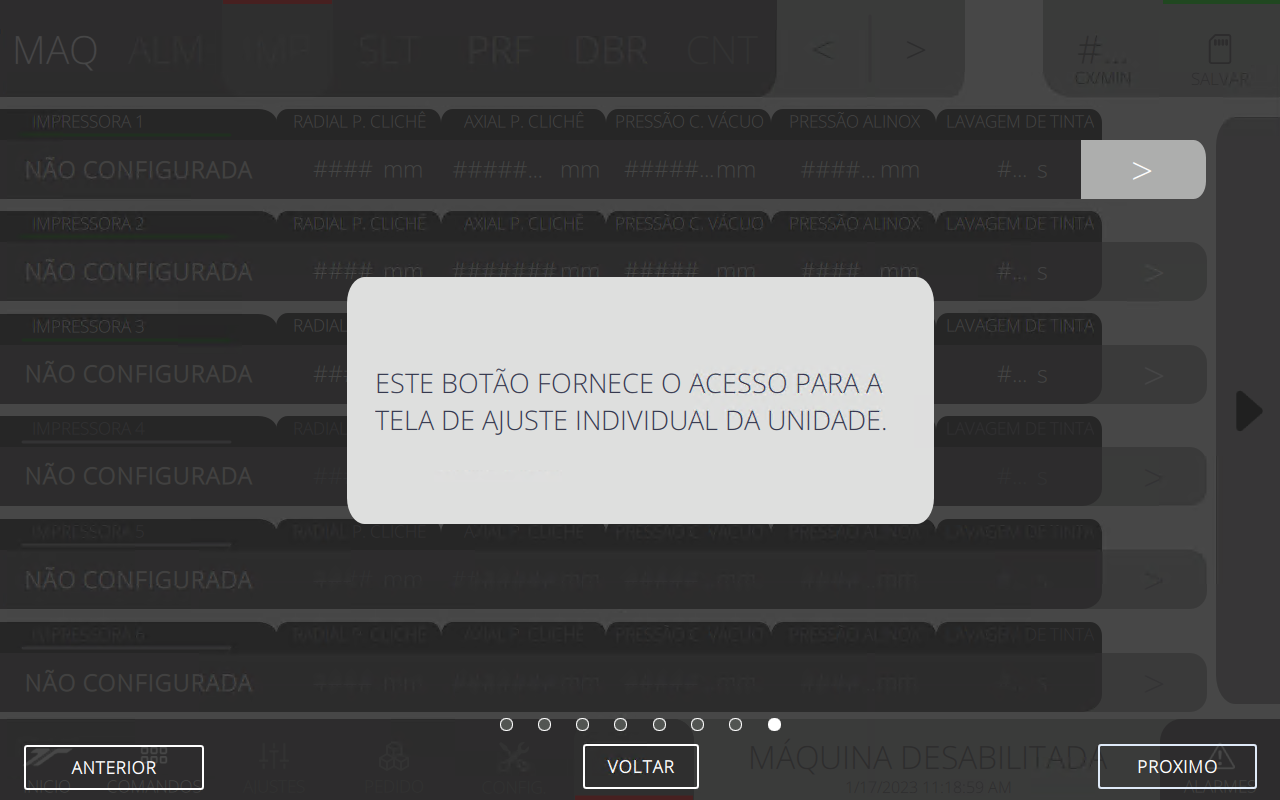
\includegraphics[width=576px,height=360px]{src/imagesFlexo/04-printter/01-printters/settings/e-8.png}
\end{figure}
\vspace*{\fill}

\newpage
\thispagestyle{fancy}
\vspace*{40 pt}
\subsection{Segunda tela de ajustes impressoras}\label{telaAjustesImpressorasSegundaTelaDeAjustesImpressoras}
Esta tela é acessada pelo botão direito "\textgreater" na tela de ajustes de \textbf{impressoras}. A lógica dos outros menus continua sendo a mesma da sua tela "pai" e para voltar a tela anterior basta clicar no botão esquerdo "\textless{}".
\vspace*{\fill}
\begin{figure}[h]
  \centering
  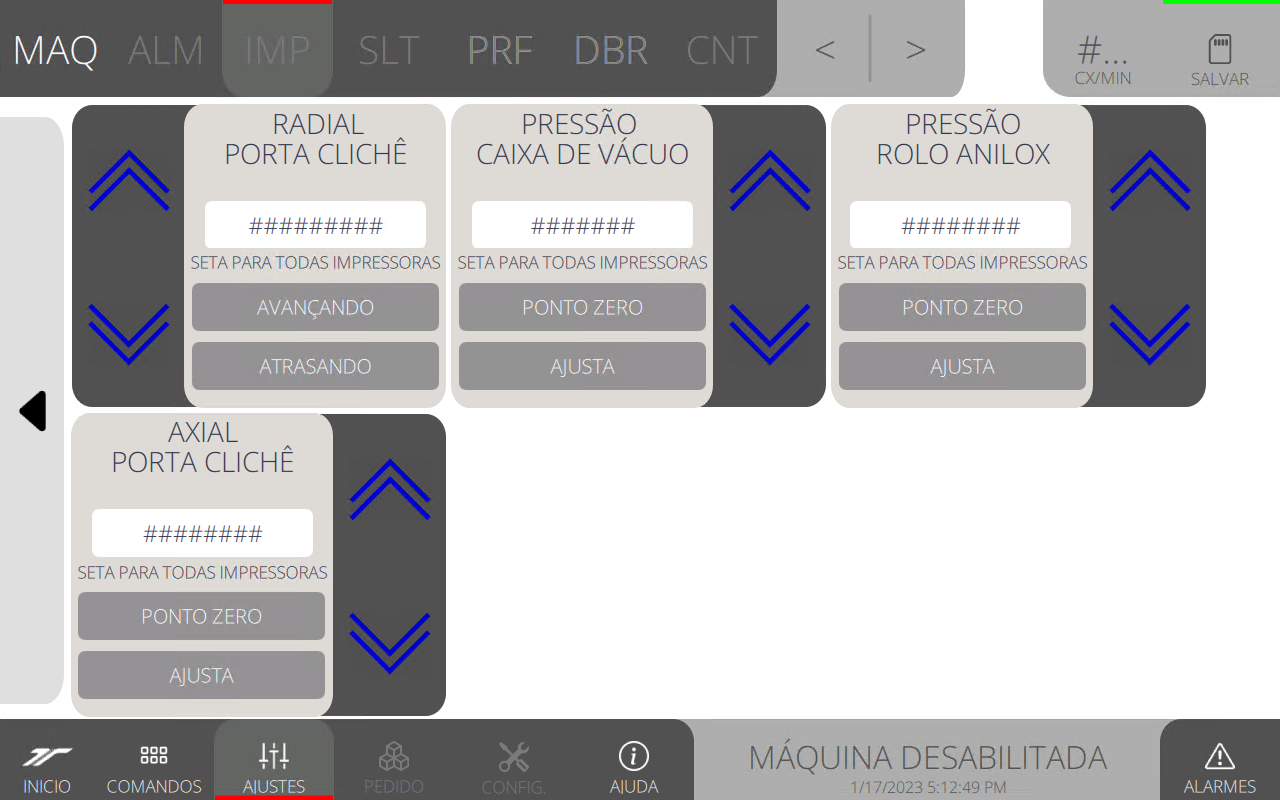
\includegraphics[width=576px,height=360px]{src/imagesFlexo/04-printter/01-printters/settings/e-Tela-Principal-2.png}
\end{figure}
\vspace*{\fill}

\newpage
\thispagestyle{fancy}
\vspace*{40 pt}
\subsubsection{\small{Ajusta posição axial porta clichê para todas as impressoras}}\label{telaAjustesImpressorasSegundaTelaDeAjustesImpressorasAjustaPosicaoAxialPortaClicheParaTodasAsImpressoras}
\vspace*{\fill}
\begin{figure}[h]
  \centering
  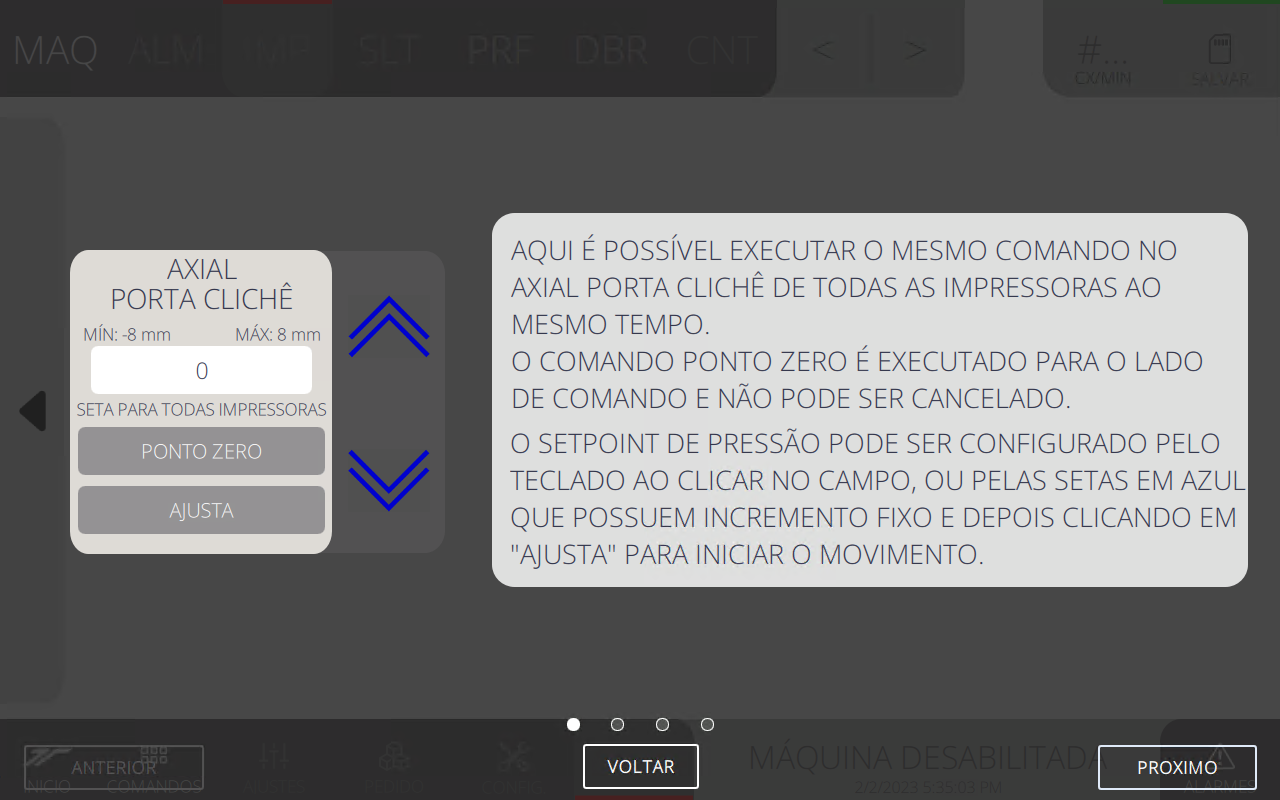
\includegraphics[width=576px,height=360px]{src/imagesFlexo/04-printter/01-printters/settings/e-9.png}
\end{figure}
\vspace*{\fill}

\newpage
\thispagestyle{fancy}
\vspace*{40 pt}
\subsubsection{\small{Ajusta pressão da caixa de vácuo para todas as impressoras}}\label{telaAjustesImpressorasSegundaTelaDeAjustesImpressorasAjustaPressaoDaCaixaDeVacioParaTodasAsImpressoras}
\vspace*{\fill}
\begin{figure}[h]
  \centering
  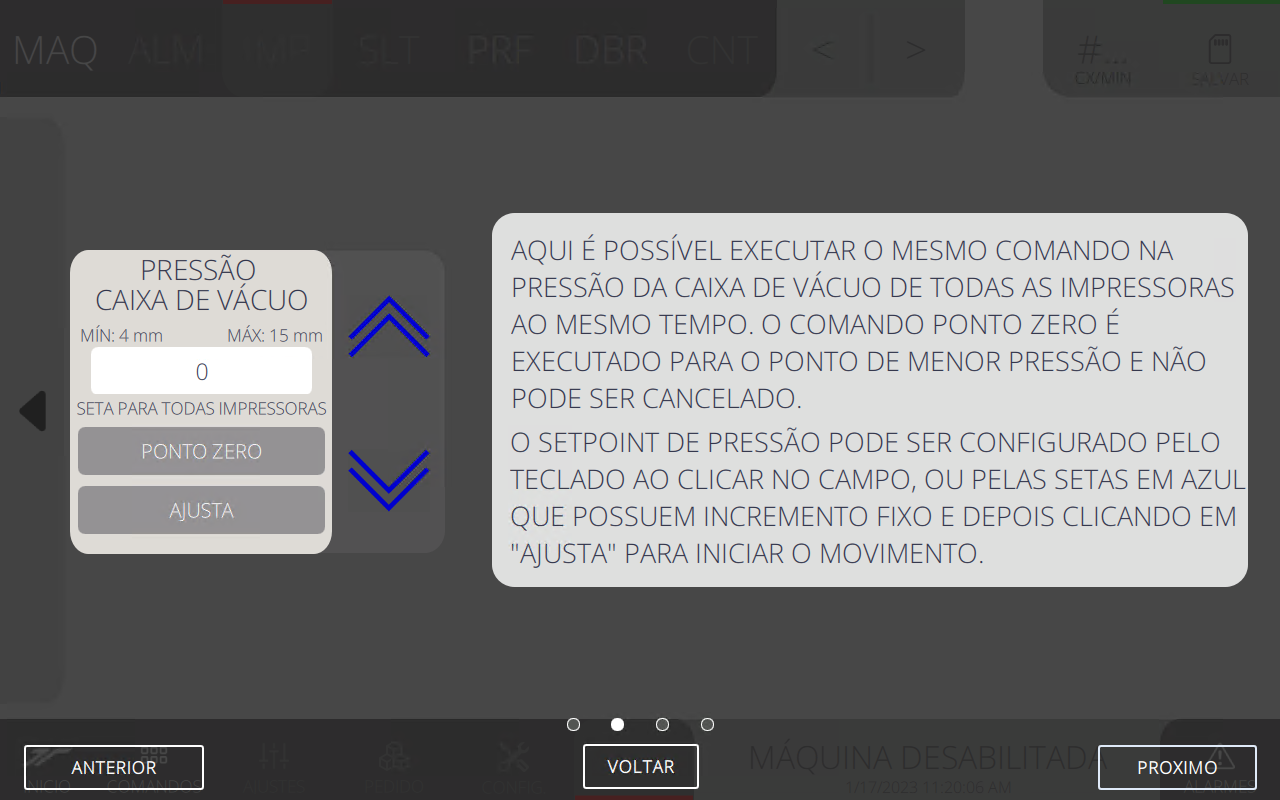
\includegraphics[width=576px,height=360px]{src/imagesFlexo/04-printter/01-printters/settings/e-10.png}
\end{figure}
\vspace*{\fill}

\newpage
\thispagestyle{fancy}
\vspace*{40 pt}
\subsubsection{\small{Ajusta registro do clichê para todas as impressoras}}\label{telaAjustesImpressorasSegundaTelaDeAjustesImpressorasAjustaRegistroDoClicheParaTodasAsImpressoras}
\vspace*{\fill}
\begin{figure}[h]
  \centering
  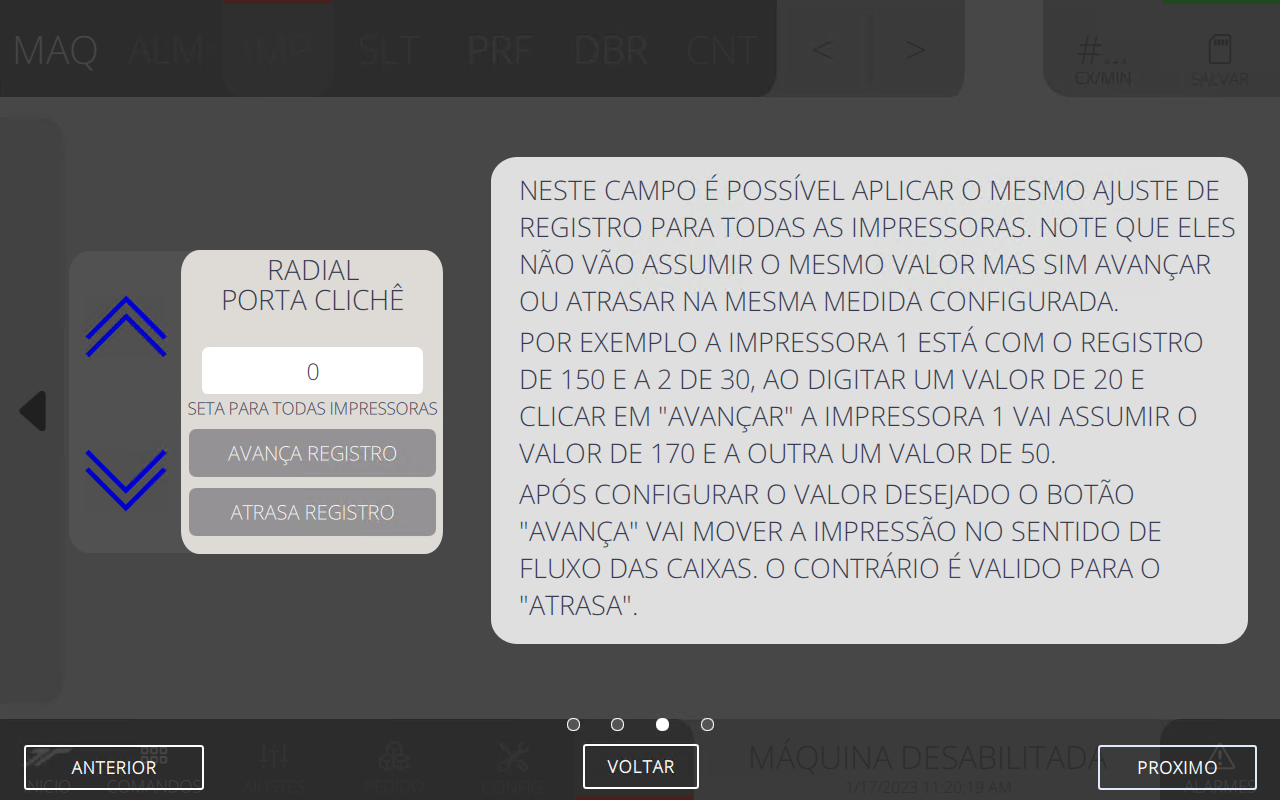
\includegraphics[width=576px,height=360px]{src/imagesFlexo/04-printter/01-printters/settings/e-11.png}
\end{figure}
\vspace*{\fill}

\newpage
\thispagestyle{fancy}
\vspace*{40 pt}
\subsubsection{\small{Ajusta pressão do rolo anilox para todas as impressoras}}\label{telaAjustesImpressorasSegundaTelaDeAjustesImpressorasAjustaPressaoDoRoloAniloxParaTodasAsImpressoras}
\vspace*{\fill}
\begin{figure}[h]
  \centering
  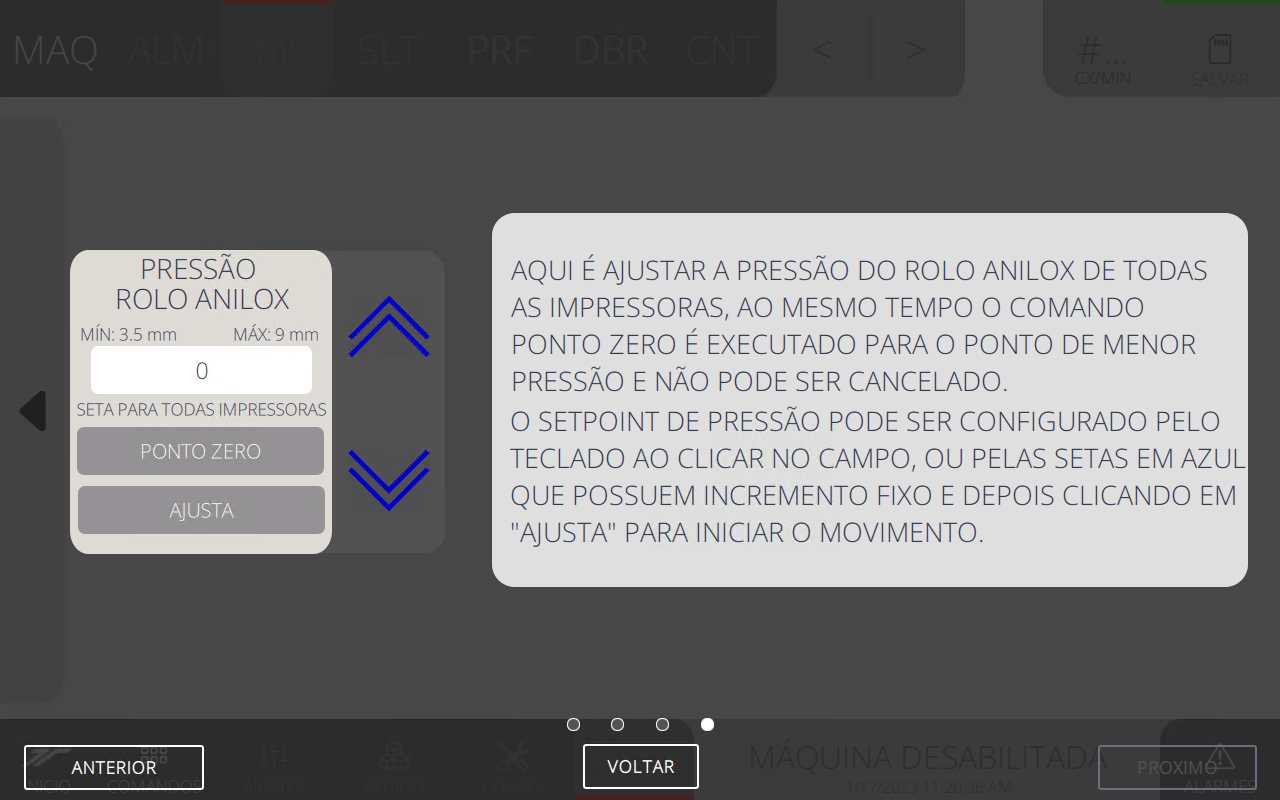
\includegraphics[width=576px,height=360px]{src/imagesFlexo/04-printter/01-printters/settings/e-12.png}
\end{figure}
\vspace*{\fill}
